% -*- latex -*-

%%%%%%%%%%%%%%%%%%%%%%%%%%%%%%%%%%%%%%%%%%%%%%%%%%%%%%%%%%%%%%%%%%%%%%%%%%%%%
% This metadata is specific for the sig-alternate document class.

\documentclass{sig-alternate}

\conferenceinfo{Ultravis}{2013 Denver, CO USA}
\CopyrightYear{2013} % Allows default copyright year (20XX) to be over-ridden - IF NEED BE.
%\crdata{0-12345-67-8/90/01}  % Allows default copyright data (0-89791-88-6/97/05) to be over-ridden - IF NEED BE.

\title{A Classification of Scientific Visualization Algorithms for Massive Threading}

% ACM has this complicated setup for authors that only really works for 6
% or less and is pretty big and pretty ugly in any case. This is amore
% compact representation.

\numberofauthors{1}

\author{
  \alignauthor
  Kenneth~Moreland,$^{\ddagger}$ Berk~Geveci,$^*$ Kwan-Liu~Ma,$^{\dagger}$
  and Robert~Maynard$^*$\\
  \affaddr{$^{\ddagger}$Sandia National Laboratories}\\
  \affaddr{$^*$Kitware, Inc.}\\
  \affaddr{$^{\dagger}$University of California at Davis}\\
}

% End of metadata specific for sig-alternate document class.
%%%%%%%%%%%%%%%%%%%%%%%%%%%%%%%%%%%%%%%%%%%%%%%%%%%%%%%%%%%%%%%%%%%%%%%%%%%%%

\usepackage{amsfonts}
\usepackage{amssymb}
\usepackage{amsmath}
\usepackage{booktabs}
\usepackage{enumitem}
\usepackage{graphicx}
\usepackage{varioref}
\usepackage{fancyvrb}
\usepackage{ifthen}
\usepackage{cite}
\usepackage{subfig}
\usepackage{tabulary}
\usepackage{xspace}
\usepackage[pdfborder={0 0 0}]{hyperref}
\usepackage{verbatim}

\usepackage{color}
\definecolor{yellow}{rgb}{1,1,0}
\definecolor{black}{rgb}{0,0,0}
\definecolor{ltcyan}{rgb}{.75,1,1}
\definecolor{red}{rgb}{1,0,0}
\definecolor{gray}{rgb}{.6,.6,.6}
\definecolor{darkred}{rgb}{0.5,0,0}
\definecolor{darkgreen}{rgb}{0,0.5,0}

% Cite commands I use to abstract away the different ways to reference an
% entry in the bibliography (superscripts, numbers, dates, or author
% abbreviations).  \scite is a short cite that is used immediately after
% when the authors are mentioned.  \lcite is a full citation that is used
% anywhere.  Both should be used right next to the text being cited without
% any spacing.
\newcommand*{\lcite}[1]{~\cite{#1}}
\newcommand*{\scite}[1]{~\cite{#1}}

\newcommand{\etal}{et al.}

\newcommand*{\keyterm}[1]{\emph{#1}}

\newcommand{\fix}[1]{{\color{red}\textsc{[#1]}}}

% Avoid putting figures on their own page.
\renewcommand{\textfraction}{0.05}
\renewcommand{\topfraction}{0.95}
\renewcommand{\bottomfraction}{0.95}

% Make sure this is big enough so that only big figures end up on their own
% page but small enough so that if a figure does have to be on its own
% page, it won't push everything to the bottom because it's not big enough
% to have its own page.
\renewcommand{\floatpagefraction}{.75}

\newenvironment{packed_itemize}{
  \begin{itemize}[noitemsep]
}{
  \end{itemize}
}

\newcommand{\algclass}[1]{\textsf{#1}}
\newcommand{\alg}[1]{#1}

%% \newcommand{\algorithmclasssection}[1]{
%%   \vspace{\baselineskip}\noindent{\large\textbf{\algclass{#1}}}}
\newcommand{\algorithmclasssection}[1]{\subsection*{#1}}

\newcommand{\algorithmclass}[7]{
  \algorithmclasssection{#1} %
  %\vspace{-.4\baselineskip}
  \begin{description}[leftmargin=10em,style=nextline,noitemsep]
    \raggedright
  \item[Separable Element] #2
  \item[Point Mapping] #3
  \item[Cell Mapping] #4
  \item[Field Mapping] #5
  \item[Collective Work] #6
  \item[Algorithms] #7
  \end{description}
}

\newcommand{\exampleimage}[2][.24]{\includegraphics[width=#1\textwidth]{images/Example#2}}

\hyphenation{Para-View Map-Re-duce}

\begin{document}

\sloppy

\maketitle

\begin{abstract}

As the number of cores in processors increase and accelerator architectures
are becoming more common, an ever greater number of threads is required to
achieve full processor utilization. Our current parallel scientific
visualization codes rely on partitioning data to achieve parallel
processing, but this approach will not scale as we approach massive
threading in which work is distributed in such a fine level that each
thread is responsible for a minute portion of data. In this paper we
characterize the challenges of refactoring our current visualization
algorithms by considering the finest portion of work each performs and
examining the domain of input data, overlaps of output domains, and
interdependencies among work instances. We divide our visualization
algorithms into eight categories, each containing algorithms with the same
interdependencies. By focusing our research efforts to solving these
categorial challenges rather than this legion of individual algorithms, we
can make attainable advancement for extreme computing.

\end{abstract}

\section{Introduction}

\noindent
Processor clock and execution rates have flatlined. Instead, successive
generations of processors provide more parallel threading
capability\lcite{Sutter2005}. Recent CPUs feature multiple cores and
hyperthreading technology to allow each core to run concurrent
threads. Furthermore, accelerator type architectures, which have
lightweight cores grouped to share control, are becoming increasingly
popular for their high ratios of price and power to performance.

High performance computing is also seeing a remarkable increase in the
parallelism required on large-scale systems. Consider, for example, the
last two generations of leadership-class computers at the Oak Ridge
Leadership Computing Facility. The previous Jaguar-XT5 system had a peak
performance of about 2 petaflops using about 200 thousand concurrent
processes. The current Titan-XK7 system, which incorporates GPU
accelerators, has a peak performance of over 20 petaflops but can require
70 to 500 \emph{million} concurrent threads in order to achieve
that. Building algorithms that are implemented for new process
architectures and programming models and that support the massive
parallelization they require is considered one of the top research
challenges for scientific visualization\lcite{Childs2013}.

Production visualization products today achieve parallel scalability using
a data parallel method that relies on partitioning the data into
independent domains for each process\lcite{Ahrens2001}. Each domain is
processed independently, so ghost regions and overlap are required at
domain boundaries so that the interaction of work on parallel processes can
be ignored. However, this approach is infeasible when dealing with massive
amounts of threads on these emerging architectures. We now need to design
new algorithms with a key on data interdependencies to process efficiently
in a massively threaded environment.

Unfortunately, to perform scientific visualization with massive threading,
we need to redesign our algorithms to work effectively with fine-grained,
independent operations. There has already been significant work in making
scientific visualization algorithms work well with shared memory threading
and accelerator types of
architectures\lcite{PISTON,Dyken2008,Maynard2013,EAVL,Meredith2012}, but
all these projects focus on the implementation of a single or select fixed
set of algorithms. Our goal in this paper is to present commonalities among
various algorithms that share parallel-programming challenges. By
addressing these higher level challenges, we can make better progress to
ensure that our scalable scientific visualization needs are met.

To identify these high level parallel-programming challenges, we first
revisit the key principles on which we base our current parallel
visualization algorithms (Section~\ref{sec:KeyPrinciples}) and then
categorize our current set of scientific visualization algorithms based on
behavior of the fundamental computation
(Section~\ref{sec:Classification}).


\section{Key Principles}
\label{sec:KeyPrinciples}

\begin{figure*}
  \centering
  \subfloat[Serial Partitioning]{
    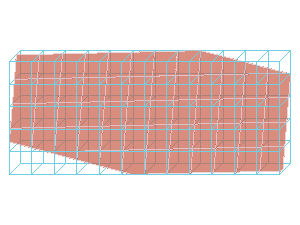
\includegraphics[scale=.9]{images/SliceSerial}
    \label{fig:Partitioning:Serial}
  }
  \subfloat[Coarse-Parallel Partitioning]{
    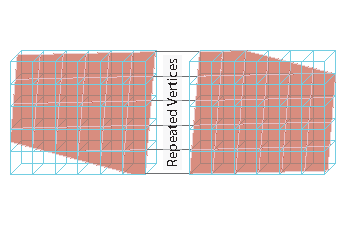
\includegraphics[scale=.9]{images/SliceCoarseParallel}
    \label{fig:Partitioning:Coarse}
  }
  \subfloat[Massively-Threaded Partitioning]{
    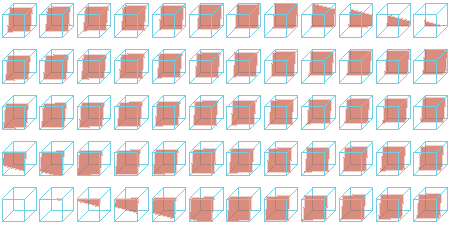
\includegraphics[scale=.9]{images/SliceMassiveThread}
    \label{fig:Partitioning:Massive}
  }
  \caption{Partitioning with different levels of parallelism. In serial
    processing~(\protect\subref*{fig:Partitioning:Serial}) geometry is
    fully connected. Partitioning for parallel processing introduces
    disconnected cells and repeated
    vertices~(\protect\subref*{fig:Partitioning:Coarse}), which become
    unmanageable in massive
    threading~(\protect\subref*{fig:Partitioning:Massive}).  }
  \label{fig:Partitioning}
\end{figure*}

\noindent
Our current scalable scientific visualization relies on a coarse
partitioning of data into domains that can often be processed
independently. Law \etal\scite{Law1999} provides the following three key
principles that must be satisfied for this independent processing to behave
correctly.

\begin{description}
\item[Data Separability] The data can be broken into domains in a way that
  is simple and efficient. Furthermore, algorithms behave properly on
  independent domains.
\item[Mappable Input] Given an identification for a portion of the output,
  the input domain responsible for this output can be determined. The
  output portion can, and often is, identified as simply piece $i$ of $N$.
\item[Result Invariant] The output of the algorithm is equivalent across
  all possible partitioning.
\end{description}

At first glance, it would appear that any algorithm abiding by these key
principles could be partitioned indefinitely. However, there are two
problems that arise when building a massively threaded algorithm in which
the data is partitioned (potentially) down to domains of single elements.

The first problem is that many algorithms do not really have a clear
mapping from an algorithm's output to its input. For example, when
computing a contour\lcite{Lorensen1987}, it is seldom practical \emph{a
  priori} to know how large the output will be, to know from what domain of
the input each piece of the output will originate, and to know what the
distribution of elements in the output partitions will be. As long as the
data partitioning is coarse enough, managing uneven or empty domains is
inconsequential. Load imbalance in downstream processing can either be
resolved by dynamic rebalancing or, more commonly, simply tolerating
it. However, to achieve efficiency with massive threading, it is important
to know the precise elements on which to schedule the working
threads. Thus, it is often more practical to determine partitioning by
mapping from input to output rather than output to input.

The second problem is that although plenty of algorithms are result
invariant in that different partitioning results are \emph{equivalent}, the
structures they build are not strictly \emph{isomorphic}. Partitioning data
often results in duplicate information on domain boundaries. Consider for
example the slice operation demonstrated in
Figure~\ref{fig:Partitioning}. In serial~(\ref{fig:Partitioning:Serial}) it
is straightforward to create a fully connected manifold surface. With
coarse level partitioning~(\ref{fig:Partitioning:Coarse}), as is typically
used in MPI processing, partitioning creates gaps between domains and
replicated vertices at the boundaries. Massive
threading~(\ref{fig:Partitioning:Massive}) can result in a completely
disconnected mesh. Although all these results are equivalent with respect
to the combined results, the different underlying data structures have
different properties and associated capabilities.

This duplication of results is a convenient mechanism to avoid
communication in parallel processing, and in coarse-level parallelism the
duplication is easily managed through ghost regions. (Anecdotally this
works best when each process has on the order of 100 thousand to 10 million
cells per process\lcite{ParaViewTutorial}) However, if massive threading
reduces each domain to every independent element, the duplication is
dramatic and creating ghost regions is infeasible. It is therefore not
practical to assume result invariance for most algorithms. Instead we have
to identify and characterize the \keyterm{interdependence} of the work
where concurrent threads produce coincident data or the threads otherwise
require collective operations. It is only then that we can design
strategies to manage the work interdependence.

With these issues in mind, we provide an analogous set of key principles
for the operation of scientific visualization algorithms for massive
threading.

\begin{description}
\item[Data Separability] The data can be broken down to an elemental level
  fine enough to provide independent work for sufficient threads.
\item[Discoverable Input Mapping] The existence of output elements can be
  efficiently determined from the input.
\item[Collective Work] In the cases where work is not independent, the
  overlap of responsibility can be resolved through efficient collective
  operations.
\end{description}


\section{Classification of Visualization Algorithms}
\label{sec:Classification}

\begin{figure*}
  \centering
  \exampleimage{Elevation}
  \exampleimage{GenerateIds}
  \exampleimage{SurfaceVectors}
  \exampleimage{Warp}
  \caption{Examples of \algclass{Basic Mapping} algorithms.}
  \label{fig:BasicMapping}
\end{figure*}

\begin{figure*}[hbt]
  \centering
  \exampleimage[.3]{CellCenters}
  \exampleimage[.3]{CellDerivatives}
  \exampleimage[.3]{MeshQuality}
  \caption{Examples of \algclass{Map by Cell} algorithms.}
  \label{fig:MapByCell}
\end{figure*}

\noindent
To better understand the effort involved with updating our scientific
visualization algorithms to massively threaded processors, we look into the
behavior of the algorithms we are currently using in production
tools. Specifically, we consider those algorithms available in ParaView, a
popular open-source scalable scientific visualization
application\lcite{ParaView}.

For each algorithm in ParaView, we apply the three key principles defined
at the end of Section~\ref{sec:KeyPrinciples}: data separability,
discoverable input mapping, and collective work. To address data
separability, we consider the smallest unit of data on which a single
thread can independently operate, which we call the \keyterm{separable
  element}. To address discoverable input mapping, we consider how the
elements of the input data map to the points and cells of the output
geometry and the output fields. Finally, we also identify any
\keyterm{collective work} the algorithm must perform in a multithreaded
environment.

From this information we derive classes of scientific visualization
algorithms where the algorithms of each class share the same input,
output, and interdependence characteristics. This classification is
constructive because once we resolve the challenges of mapping input to
output and managing interdependence with collective operations, the
algorithms within each class are straightforward to implement from their
serial counterparts. A reference for all these classifications is given at
the end of this paper in Table~\ref{table:Classifications}.

\algorithmclass{Basic Mapping}
               {Any} % Separable Element
               {Identity} % Point Mapping
               {Identity} % Cell Mapping
               {1 to 1} % Field Mapping
               {None} % Collective Work
               {
                 Append Attributes,
                 Append Datasets,
                 Calculator,
                 Elevation,
                 Generate Ids,
                 Image/Rectilinear Data to Point Set,
                 Random Vectors,
                 Reflect,
                 Surface Vectors,
                 Texture Map Coordinates,
                 Transform,
                 Warp
               }

\noindent
The \algclass{Basic Mapping} algorithms operate on an array of field values
and generate another array of field values. Each output field value is
computed independently using only the associated input value (or values if
there is more than one input array).

The typical purpose of this type of algorithm is to generate a derived
field of data. Some of these operate on the coordinates of mesh points, for
example the \alg{Transform} filter moves and warps the data with an affine
transformation. However, when point coordinates are treated as a field, the
behavior characteristics are the same. Some examples of \algclass{Basic
  Mapping} algorithms are given in Figure~\ref{fig:BasicMapping}. The
example shuttle data is courtesy of the NASA Advanced Supercomputing
Division.

The \algclass{Basic Mapping} class is essentially just a parallel
\texttt{for} operation over input and output field arrays. As such, basic
mapping is essentially built in to many multi- and many-core languages and
APIs including OpenMP (parallel for pragma\lcite{Quinn2004}), CUDA (triple
chevron notation\lcite{Sanders2011}), Thrust (for\_each generic
algorithm\lcite{Thrust}), and Intel Threading Building Blocks
(parallel\_for generic algorithm\lcite{TBB}). Although all of these systems
use significantly different syntax, Baker \etal\scite{Baker2010} show how
to simplify porting using a generic programming interface over them.


\algorithmclass{Map by Cell}
               {Cell} % Separable Element
               {Identity} % Point Mapping
               {Identity} % Cell Mapping
               {Points on cell to cell} % Field Mapping
               {None} % Collective Work
               {
                 Cell Centers,
                 Cell Derivatives,
                 Mesh Quality,
                 Point Data to Cell Data
               }

\noindent
The \algclass{Map by Cell} class is very similar to \algclass{Basic
  Mapping} with the exception that the input field arrays are not a
one-to-one mapping to the output field arrays. Instead, these operations
are performed using the information over a complete cell and attached
fields.

Operations of this class involve characterizing the shape of the cell (as
in the case of \alg{Cell Centers} and \alg{Mesh Quality}) or math
operations over continuous function rather than discrete values (as is the
case for \alg{Cell Derivatives}). Some examples of \algclass{Map by Cell}
are given in Figure~\ref{fig:MapByCell}.

Although parallel threads generally do access overlapped portions of the
input data, the calculations computed by each thread are independent and
there is no overlap in the output they produce and are thus easy to
parallelize. The EAVL library and Dax toolkit each provide a generic
algorithm to perform \algclass{Map by Cell}\lcite{EAVL,Moreland2011:LDAV}.


\algorithmclass{Reconnect Cell}
               {Cell} % Separable Element
               {1 to 0 or 1} % Point Mapping
               {1 to 0 or more} % Cell Mapping
               {Identity} % Field Mapping
               {None} % Collective Work
               {
                 Extract Cells by Region,
                 Extract Selection,
                 Mask Points,
                 Tetrahedralize,
                 Threshold,
                 Triangulate
               }

\begin{figure*}
  \centering
  \exampleimage[.43]{Extract}
  \exampleimage[.43]{Threshold}
  \caption{Examples of \algclass{Reconnect Cell} algorithms.}
  \label{fig:ReconnectCell}
\end{figure*}

\begin{figure*}
  \centering
  \exampleimage{Glyph}
  \exampleimage{Ribbon}
  \exampleimage{Shrink}
  \exampleimage{Tube}
  \caption{Examples of \algclass{Build Independent Topology} algorithms.}
  \label{fig:BuildIndependentTopology}
\end{figure*}

\noindent
There are several apparent patterns in algorithms that build a topological
structure, the first of which is \algclass{Reconnect Cell}. The
characteristics of these algorithms are that the output topology uses the
same points as (or a subset of the points from) the input topology and that
each output cell depends on exactly one input cell. In essence the
connectivity of each cell is being redefined. Some examples of
\algclass{Reconnect Cell} algorithms are given in
Figure~\ref{fig:ReconnectCell}.

Because each thread creates an independent list of cell connections,
\algclass{Reconnect Cell} algorithms have no interdependence. This makes
them very similar to \algclass{Map by Cell} algorithms with the important
exception that most \algclass{Reconnect Cell} algorithms have a variable
number of outputs across the threads that is not known at the onset of
execution. Thus, these algorithms must implement some form of
\keyterm{stream compaction} to build efficient packed arrays for the
output. Also, since some of these algorithms only use a subset of the input
points, it may be desirable to explicitly identify and extract these
points.

Each of the three SDAV many-core frameworks for
visualization\lcite{Sewell2012} provides an example of \alg{Threshold}, a
\algclass{Reconnect Cell} algorithm, using a different approach. PISTON
uses a stream compaction algorithm to determine an efficient output layout
and then generates the output cells in parallel\lcite{PISTON}. New points
are created in the output, which implicitly removes points from the input
at the expense of replicating points in the output. Dax uses a similar
stream compaction but outputs a more compact array of connection
identifiers\lcite{Maynard2013}. Dax can also optionally extract the subset
of points used in the output at an added computational expense. EAVL
provides a different approach wherein the output data structure references
the input structure and the data management makes this behave as an
independent data structure\lcite{Meredith2012}. This approach is much
faster and memory efficient, but there is no explicit representation of the
result for use in other packages that might expect that and it is not
possible to remove the input structure from memory as long as the output
still references it.


\algorithmclass{Build Independent Topology}
               {Any} % Separable Element
               {1 element to many points} % Point Mapping
               {1 element to many cells (constant number)} % Cell Mapping
               {Identity} % Field Mapping
               {None} % Collective Work
               {
                 Glyph,
                 Ribbon,
                 Shrink,
                 Tube
               }

\noindent
Algorithms that \algclass{Build Independent Topology} create new geometry
requiring both new points and new cells that connect these points. The
geometry created by each thread in this algorithm class is completely
independent from that created in any other thread; there are no topological
connections between them.

For example, consider the \alg{Glyph} filter. Each thread in this filter
produces a small 3D object, like a scaled sphere or oriented arrow,
centered at the point assigned to the thread. Each 3D object is completely
disconnected (topologically) from its brethren and thus can be created
independently and concurrently. Another example is the \alg{Shrink} filter,
which contracts each cell toward its local center creating new points and
intentionally breaking connections. These and other examples of
\algclass{Build Independent Topology} algorithms are shown in
Figure~\ref{fig:BuildIndependentTopology}.

The behavioral characteristics of the \algclass{Build Independent Topology}
algorithms are very similar to the \algclass{Basic Mapping} and
\algclass{Map by Cell} algorithms. The only meaningful difference between
them is the interpretation of the output data. Instead of producing a
single or set of field values, \algclass{Build Independent Topology}
algorithms produce topologies of cells, vertices, and point coordinates;
these data must be interpreted and managed as such.


\begin{figure*}
  \centering
  \exampleimage[.31]{Clip}
  \exampleimage[.31]{Contour}
  \exampleimage[.31]{Slice}
  %% \exampleimage{Tessellate}
  \caption{Examples of \algclass{Build Connected Topology} algorithms.}
  \label{fig:BuildConnectedTopology}
\end{figure*}

\begin{figure*}
  \centering
  \exampleimage{ExtractEdges}
  \exampleimage{FeatureEdges}
  \exampleimage{Gradient}
  \exampleimage{Normals}
  \caption{Examples of \algclass{Capture Cell Adjacencies} algorithms.}
  \label{fig:CaptureCellAdjacencies}
\end{figure*}

\algorithmclass{Build Connected Topology}
               {Cell} % Separable Element
               {1 cell to 0 or more points} % Point Mapping
               {1 to 0 or more} % Cell Mapping
               {Interpolated points} % Field Mapping
               {Resolve duplicate points} % Collective Work
               {
                 Clean,
                 Clip,
                 Contour,
                 Extrusion,
                 Isovolume,
                 Slice,
                 Subdivision,
                 Tessellate
               }

\noindent
The most technically complicated class of algorithms we find that generate
geometry are those that \algclass{Build Connected Topology}. Some examples
are given in Figure~\ref{fig:BuildConnectedTopology}. These algorithms
create new geometry requiring both new points and new cells that connect
these points. The points created by each thread are coincident with points
created by another thread. These coincident points represent connections
across elements created by different threads; capturing these connections
creates an interdependence across threads.

The easiest solution to this problem is to simply ignore it by letting
coincident points exist and losing the topological connections. Thus, the
output of the algorithm is topologically a set of disconnected cells, often
referred to as a \keyterm{soup}. We find this approach common, particularly
in implementations of \alg{Contour} for
GPUs\lcite{PISTON,Dyken2008,Pascucci2004,Klein2004}.

Producing a soup of cells may be an acceptable solution in some situations,
particularly if the result is to be rendered and then forgotten, but can
also be a problematic solution. The first problem is that this redundancy
causes an inflation of the memory required. The second problem is that
subsequent algorithms, such as estimating smooth normals on a contour,
might require the lost topological connections. Existing tools,
particularly those built on VTK\lcite{VTK}, expect chains of algorithms of
this nature to work.

A typical approach to finding coincident points in a serial algorithm is to
use an iterative \keyterm{locator} structure to find any coincident points
that are already created\lcite{VTKUsersGuide}. However, this approach is
unlikely to work in a massively threaded environment as constant updates to
the locator will require far too much synchronization. Bell\scite{Bell2010}
informally proposes a \keyterm{vertex welding} algorithm that can
efficiently find these coincident points on massive threading after the
fact, but a solution working more closely to the algorithm might have
better results.


\algorithmclass{Capture Cell Adjacencies}
               {Point, edge, or face} % Separable Element
               {Identity} % Point Mapping
               {Identity} % Cell Mapping
               {Interpolated incident fields} % Field Mapping
               {Find incidence relationships} % Collective Work
               {
                 Curvature,
                 Cell Data to Point Data,
                 Extract Edges,
                 Extract Surface (external faces),
                 Feature Edges,
                 Gradient,
                 Normal Generation,
                 Smooth
               }

\noindent
The previously listed algorithms all operate on a single point in the mesh
or on a single cell and its incident features. These data are quickly
locatable in general data structures. However, some algorithms need to
\algclass{Capture Cell Adjacencies}. They typically operate by considering
the points, edges, or faces in the mesh and examining the cells incident to
them. Some examples of such algorithms are given in
Figure~\ref{fig:CaptureCellAdjacencies}.

In some types of data, particularly structured data with implicit
topologies, enumerating the mesh elements and finding incident cells is
trivial. However, in unstructured data represented by cell connection
lists, this information is not explicitly stored. Thus, although the
computation of \algclass{Capture Cell Adjacencies} algorithms are
completely independent, they might require a collective operation to
identify the domain of the input each thread needs.

Serial VTK algorithms support cell adjacencies by building a
\keyterm{links} array that lists which cells each point is incident
on\lcite{VTKUsersGuide}. A similar array could be used in a massively
threaded environment, but since a links array is not always available, we
first need an efficient massively threaded algorithm to build one.

An alternate approach is to use a different cell representation that does
explicitly capture these incidence relationships. Such alternate
representations include half-edge structures\lcite{Kettner1998}, cellular
data structures\lcite{Alumbaugh2005}, and circular incident edge
lists\lcite{Levy2001}. The drawback to these linked representations is that
storing links to every desired incidence relationship is costly. Also, most
existing data representations, including CGNS\lcite{CGNS}, VTK\lcite{VTK},
and XDMF to name a few, use cell connection lists, so a links array would
likely need to be built to convert between the representations anyway.


\algorithmclass{Globally Reduce}
               {Any} % Separable Element
               {None in output} % Point Mapping
               {None in output} % Cell Mapping
               {All to 1} % Field Mapping
               {Global reduction} % Collective Work
               {
                 Histogram,
                 Integrate,
                 Outline,
                 Statistics
               }

\noindent
Some scientific visualization algorithms perform an aggregation on the
data, often performing an operation like sum or average on a field or
derived field in the data. Thus, these algorithms \algclass{Globally
  Reduce} data into a single value or small set of values.

Reduction is a common operation in general parallel computing, and a
reduction operation is ubiquitously supported across parallel computing
environments\lcite{MPI,Sanders2011,Thrust,TBB,Quinn2004}. Consequently,
once the reduction operation can be expressed in terms of an associative
binary operation, implementing the reduction is straightforward. The
reduction is complicated slightly on a hybrid parallel machine with
multiple many-core machines clustered with an interconnect, but the
reduction can still be performed by first reducing locally within the
shared-memory many-core machine and then reducing those values across the
distributed-memory interconnect\lcite{Dinan2010}.


\algorithmclass{Query Data}
               {Point, key, or query} % Separable Element
               {Identity} % Point Mapping
               {Identity} % Cell Mapping
               {1 query to 1 output} % Field Mapping
               {Building query structure} % Collective Work
               {
                 Particle Tracer,
                 Probe Location,
                 Quadric Clustering,
                 Resample with Dataset,
                 Stream Tracer,
                 Streaklines
               }

\begin{figure}[b]
  \centering
  \exampleimage[.4]{StreamTracer}
  \caption{An example of a \algclass{Query Data} algorithm.}
  \label{fig:QueryData}
\end{figure}

\noindent
Most scientific visualization algorithms operate on a domain that is easily
identifiable by the enumeration of the work (i.e. the point or cell
identifier used to number threads). However, some algorithms must
\algclass{Query Data} to find a region of interest. Typically this means
finding a cell containing a given coordinate in space. This is part of the
fundamental operation of algorithms such as those based on resampling and
particle advection. (Note that query only solves the challenge of finding a
single integration step in particle advection, shown in
Figure~\ref{fig:QueryData}. It also needs to iterate, to connect successive
computations, and to find terminations, but these can be straightforward
extensions of existing algorithms.) Although spatial queries are common,
queries for a more general set of attributes can also be needed when
performing query-based
visualization\lcite{Glatter2008,Gosink2008,Johnson2009,Rubel2008}.

Some queries, such as a spatial query on a uniform rectilinear grid, are
straightforward, but many will require a specialized search
structure. Several spatial search structures are
proposed\lcite{Foley2005,Kalojanov2009,Kalojanov2011,Zhou2008,Zhou2010},
most for the purpose of rendering, but there is yet little research on the
building and using of query structures on massive threading for the
purposes of scientific visualization.


\begin{table*}
  \centering
  \caption{Overview of visualization algorithm classifications}
  \label{table:Classifications}
  \setlength{\defaultaddspace}{0.35\baselineskip}
  \begin{tabulary}{\textwidth}{@{}LLLLLLL@{}}
    \toprule
    Name
    & Separable Element
    & Point Mapping
    & Cell Mapping
    & Field Mapping
    & Collective Work
    & Example Algorithm \\

    \midrule

    \algclass{Basic Mapping}
    & Any
    & Identity
    & Identity
    & 1 to 1
    & None
    & \alg{Generate Ids} \\ \addlinespace

    \algclass{Map by Cell}
    & Cell
    & Identity
    & Identity
    & Points on cell to cell
    & None
    & \alg{Cell Centers} \\ \addlinespace

    \algclass{Reconnect Cell}
    & Cell
    & 1 to 0 or 1
    & 1 to 0 or more
    & Identity
    & None
    & \alg{Threshold} \\ \addlinespace

    \algclass{Build Independent Topology}
    & Any
    & 1 element to many points
    & 1 element to many cells
    & Identity
    & None
    & \alg{Glyph} \\ \addlinespace

    \algclass{Build Connected Topology}
    & Cell
    & 1 cell to 0 or more points
    & 1 to 0 or more
    & Interpolated points
    & Resolve duplicate points
    & \alg{Contour} \\ \addlinespace

    \algclass{Capture Cell Adjacencies}
    & Point, edge, or face
    & Identity
    & Identity
    & Interpolated incident fields
    & Find incidence relationships
    & \alg{Normal Generation} \\ \addlinespace

    \algclass{Globally Reduce}
    & Any
    & None in output
    & None in output
    & All to 1
    & Global reduction
    & \alg{Histogram} \\ \addlinespace

    \algclass{Query Data}
    & Point, key, or query
    & Identity
    & Identity
    & 1 query to 1 output
    & Building query structure
    & \alg{Stream Tracer} \\

    \bottomrule
  \end{tabulary}
\end{table*}


\algorithmclasssection{Remaining Algorithms}

\noindent
The previous classification of algorithms contains the majority of
algorithms in the ParaView application. There are some algorithms we have
left out of this list for a variety of reasons, which we capture here.

A very small number of algorithms have complicated interaction that appears
to be unique to the nature of the operation. The \alg{Connectivity}
algorithm needs to traverse large neighborhood regions to find connected
components. The \alg{Delaunay} algorithm needs to find all circles or
spheres containing exactly 3 or 4 points, respectively. The \alg{Halo
  Finder} algorithm identifies collections of points in mutual
proximity. The \alg{Decimate} algorithm reduces the size of geometry by
removing points based on an error metric. The \alg{Triangle Strips}
algorithm finds connected strips in triangle meshes.

There may be commonalities among some of these algorithms, but we are
unsure if these similarities extend to shared solutions for
interdependence.  Regardless, there are few algorithms with unique thread
interaction, so addressing these independently is much more tractable than
reimplementing every algorithm in existence today.

We have left out one or more classes involving imaging algorithms. These
include algorithms involving kernel convolutions and \alg{FFT}. Although
this is generally an important class of algorithms, it is not one that is
extensively used by ParaView users. The field of imaging algorithms is very
broad and of interest across many disciplines. It deserves its own study,
and thus we consider it out of the scope of this paper.

Another algorithm we have left out is \alg{Extract Subset}, which extracts
a region of interest and optionally regularly subsamples structured
data. The operation is similar to that of \algclass{Reconnect Cell} except
that the basic implementation of copying subarrays is so simplistic we omit
it.

There are several algorithms in ParaView that do not translate to running
on massive threads. Some of these algorithms do trivial metadata
manipulations like extracting a block from an assembly. Other algorithms
perform ordinary operations while making temporal
adjustments\lcite{Biddiscombe2007} or other changes to pipeline execution
management\lcite{Moreland2013:TVCG}. Also, although the \alg{Distributed
  Data Decomposition} (\alg{D3}) and similar redistribution algorithms can
be compute intensive, their data partitioning makes little sense on the
fine level dictated by massive threading.

Finally, to avoid being overly pedantic, we omit several algorithms that
are variations of algorithms listed or specialized combinations of
algorithms listed. For example, ParaView contains seven different versions
of \alg{Generate Ids} where each extracts information from different
enumerations. ParaView also has four different versions of \alg{Slice},
which have some optimizations for different data structures. There are also
several algorithms such as \alg{Material Interface} and \alg{Surface Flow}
that are each basically a conglomeration of other algorithms listed here.
It would be unnecessarily distracting to enumerate each of these
variations.


\section{Conclusion}
\label{sec:Conclusion}

\noindent
Although we have made progress in designing massively threaded
visualization algorithms for scientific visualization, we have a long way
to go to support production visualization at extreme scale. Our current
scientific and visualization needs incorporate the inclusion of many
algorithms including those designed specifically for a specialized
scientific domain. We as a community simply do not have the resources to
independently address all of these needs.

The development of our current petascale visualization tools is made
possible by observations that allow us to design a general parallel
capability that is then shared among many visualization categories. If we
cannot find a similar way to localize and reuse the parallel portion of our
algorithms, we cannot succeed in supporting the next generation of parallel
computing.

In this paper we have identified eight categories of shared features among
these algorithms summarized in Table~\ref{table:Classifications}. By
addressing the group of algorithms in each category as one, we can quickly
achieve our goal of supporting extreme scale computing.


\section{Acknowledgments}

\noindent
This work was supported in part by the DOE Office of Science, Advanced
Scientific Computing Research, under award number 10-014707, program
manager Lucy Nowell.

This work was supported in part by the Director, Office of Advanced
Scientific Computing Research, Office of Science, of the U.S. Department of
Energy under Contract No. 12-015215, through the Scientific Discovery
through Advanced Computing (SciDAC) Institute of Scalable Data Management,
Analysis and Visualization.

Sandia National Laboratories is a multi-program laboratory operated by
Sandia Corporation, a wholly owned subsidiary of Lockheed Martin
Corporation, for the U.S. Department of Energy's National Nuclear Security
Administration.

\noindent
{\small SAND 2013-7493C}


\bibliographystyle{abbrv}
\bibliography{MassivelyThreadedVis}

\end{document}
